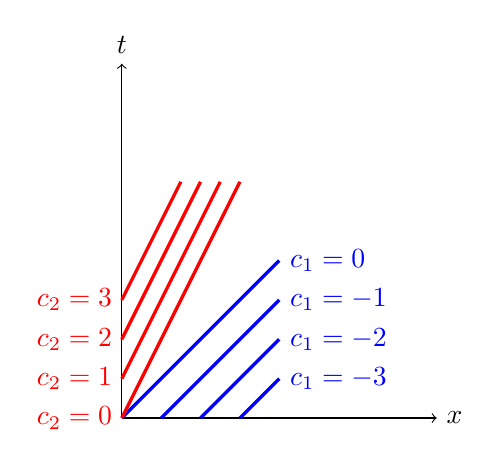
\begin{tikzpicture}
  \draw[->] (0,0) -- (4.,0) node[right] {$x$};
  \draw[->] (0,0) -- (0,4.5) node[above] {$t$};
  \draw[scale=0.5,domain=0:4,smooth,variable=\x,Blue,very thick] plot ({\x},{\x}) node [right] {$c_1=0$};
  \draw[scale=0.5,domain=1.:4,smooth,variable=\x,Blue,very thick] plot ({\x},{\x-1}) node [right] {$c_1=-1$};
  \draw[scale=0.5,domain=2:4,smooth,variable=\x,Blue,very thick] plot ({\x},{\x-2}) node [right] {$c_1=-2$};
  \draw[scale=0.5,domain=3:4,smooth,variable=\x,Blue,very thick] plot ({\x},{\x-3}) node [right] {$c_1=-3$};
  \draw[scale=0.5,domain=0:3,smooth,variable=\x,Red,very thick] plot ({\x},{2*\x});
  \node[left,Red] at (0,0) {$c_2=0$};
  \draw[scale=0.5,domain=-0.:2.5,smooth,variable=\x,Red,very thick] plot ({\x},{2*\x+1});
  \node[left,Red] at (0,0.5) {$c_2=1$};
  \draw[scale=0.5,domain=-0:2,smooth,variable=\x,Red,very thick] plot ({\x},{2*\x+2});
  \node[left,Red] at (0,1) {$c_2=2$};
  \draw[scale=0.5,domain=-0:1.5,smooth,variable=\x,Red,very thick] plot ({\x},{2*\x+3});
  \node[left,Red] at (0,1.5) {$c_2=3$};
\end{tikzpicture}
%%% Local Variables:
%%% mode: latex
%%% TeX-master: "../../mainManuscript"
%%% End:
